\section{Results}\label{sec:results}

\subsection{Overall, No Index, 3 Nodes}\label{subsec:overallNoIndex3Nodes}
\begin{figure}
    \centering{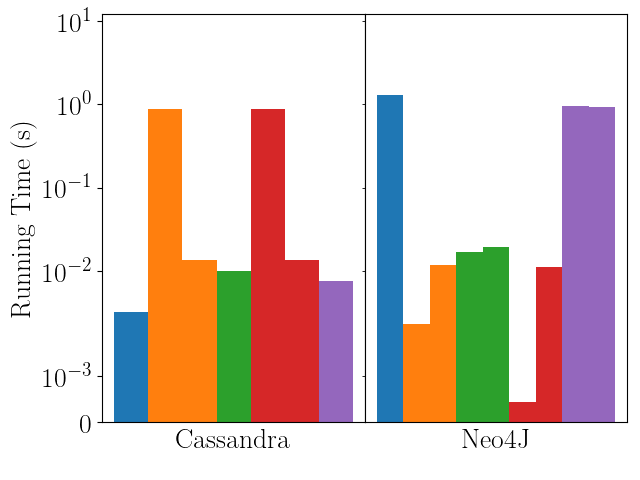
\includegraphics[scale=0.55]{images/qall-3node-none.png}}
    \caption{Running times of different queries for a 3-node Neo4J cluster and a 3-node Cassandra cluster.
    Each point represents the average of 15 runs.
    The blue bars represent query 1, the orange represent queries 2A and 2B, the green represent queries 3
    (Cassandra), 3A, and 3B (Neo4J), the red represents queries 4A and 4B, and the purple represent queries 5
    (Cassandra), 5A, and 5B (Neo4J).}\label{fig:ono3n}
\end{figure}

In~\autoref{fig:ono3n}, all queries are plotted against time for both Neo4J and Cassandra.
Each cluster consists of 3 nodes, and no indexes are applied to any column.

Neo4J performs better with queries given some position $(\alpha, \delta)$, while Cassandra performs better with
queries given the \texttt{TYC} ID\@.
Given that the Cassandra families are not indexed by their Equatorial position columns, it makes sense
that Neo4J would shine here.
For queries 2A and 4A, Neo4J performs an average of 0.88s faster than Cassandra.
For queries 1, 3 (3A for Neo4J), and 5 (5A for Neo4J), Cassandra performs an average of 1.27s faster.
Cassandra query 3 takes about the same time to run as Neo4J query 3A, at a difference of $\sim$7.9ms.

Neo4J's significant change in running time from query 3A to 5A is interesting, as the only change made is
applying a brightness filter.
Running both query sets through Neo4J's query planner reveals that query 3A is \textit{compiled} and 5A is
\textit{slotted}.
A compiled Neo4J query groups operators in the execution plan to optimize performance and memory usage, while a
slotted query only optimizes how records are fed into each iterator.
It appears that the inclusion of this brightness filter prevents query 5A from being compiled and optimizing
performance.
Running several queries from query set 1 through the query planner shows that this is also compiled, but is still
slower than query set 3A\@.
The main difference here is the inclusion of two more filters (\texttt{TYC2} and \texttt{TYC3}), which might explain
this difference in time.

For both Cassandra and Neo4J, queries 2A, 4A, and 2B, 4B differ in their approach to determine the region our star is
in.
Reading a file containing the region data and determining our \texttt{TYC1} in application logic instead of
performing the exhaustive search on our \textit{Region} family does yield a time decrease of 0.87s.
For the non-indexed Neo4J, this approach has no significant effect on performance (average of 8.31ms increase).
Given that no mechanisms are in place for Neo4J to take advantage of this, it makes sense that no speed up is shown.

In Neo4J queries 3B and 5B, we vary our query to include the \textit{Region} node as opposed to their A variants.
Both require a full search of the entire \textit{Star} node list, but the B queries require an additional traversal
to the matching \textit{Region} node and additional hops to each \textit{Star} node.
These additional steps suggest that the A queries should be faster, but the results are mixed.
Our results show that query 3A takes the same amount of time to run as query 3B (9.68ms difference), while query 5B
is actually $\sim$69ms faster than 5A\@.

%The query planner for each of these queries are as follows:
%\begin{itemize}
%    \item[1)] Gather all \textit{Star} nodes $\rightarrow S$
%    \item[2a)] ID filter ($i$): $\{ S \mid S.\texttt{TYC1} = i\} \rightarrow S'$
%    \item[2b)] Brightness filter ($m$): $\{ S' \mid S'.\texttt{BTmag} < m\} \rightarrow S''$
%    \item[3)] Present our result $S'$ or $S''$
%\end{itemize}
%Query 3A is the least restrictive

In terms of query time distribution, the average deviation of all Cassandra queries is 20.4ms, while the average Neo4J
deviation is 3.36s.
Neo4J queries can take up to 2 minutes to return a single result, and under a second for others.
On average, our Cassandra cluster performs all queries faster than our non-indexed Neo4J cluster by 0.13s.

\subsection{Queries \{1, 3, 5\}, TYC Index, 3 Nodes}\label{subsec:queries135TycIndex3Nodes}
\begin{figure}
    \centering{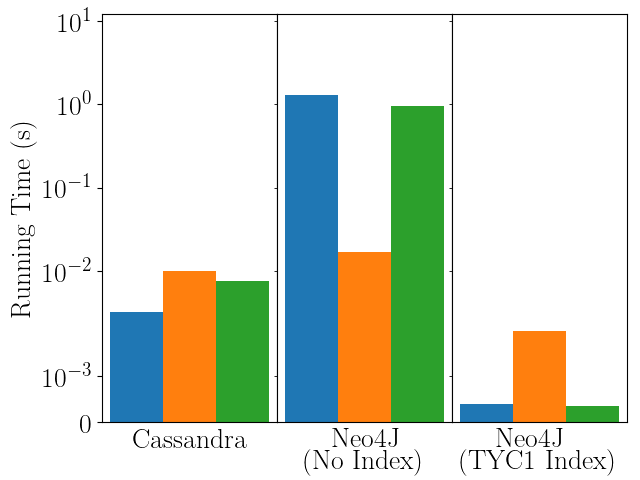
\includegraphics[scale=0.55]{images/q135-3node-tycindex.png}}
    \caption{Running times of queries 1, 3, and 5 for a 3-node Cassandra cluster, a 3-node Neo4J cluster without an
    index on \texttt{TYC1}, and another 3-node Neo4J cluster with the specified index.
    Each point represents the average of 15 runs.
    The blue bars represents query 1, the orange represents query 3 (3A for Neo4J), and the green represents query 5
    (5A for Neo4J).}\label{fig:1qtycindex3n}
\end{figure}

In~\autoref{fig:1qtycindex3n}, queries 1, 3 (3A for Neo4J), and 5 (5A for Neo4J) are plotted for a 3-node Cassandra
cluster, a 3-node Neo4J cluster without any indexes, and a 3-node Neo4J cluster with an index on \texttt{TYC1}.
All of three of these queries involve searching for some star based on the \texttt{TYC1} field.
The \texttt{TYC1} index cannot be applied to our Cassandra cluster because this is the primary key for \textit{Stars}
column family.

On average, the \texttt{TYC1} indexed Neo4J cluster performs about the same as our current Cassandra cluster
($\sim$6ms difference).
Cassandra performs 0.85s faster than a non-indexed Neo4J cluster.
The average difference in time between the non-indexed Neo4J cluster and the \texttt{TYC1} indexed cluster is 0.85s.
The inefficiencies seen in~\autoref{subsec:overallNoIndex3Nodes} for Neo4J queries 1 and 5A are reduced with the
inclusion of an index on the filtered field.

Relative to queries 1 and 5, query 3 was already fast (average of 1.27s vs. $\sim$18ms).
After applying the index, query 3 becomes the slowest of the three, although the difference is fairly small (1.6ms).
Query 3B is also more distributed than queries 1 and 5A (0.96ms vs. 0.06ms), suggesting that this behaviour is
consistent.

A slight performance boost may be gained for both query 1s of Neo4J if a size restriction filter were placed (i.e.
\texttt{LIMIT}).
For the non-indexed case, this query is of complexity $T(n) = \Theta(n)$ and could be lowered to $O(n)$ if we
restrict our resultant to one element.

\subsection{Queries \{4, 5\}, BTmag Index, 3 Nodes}\label{subsec:queries45btmagIndex3Nodes}
\begin{figure}
    \centering{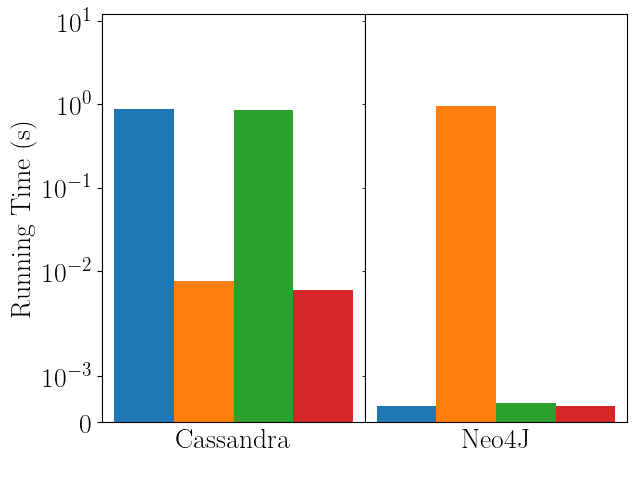
\includegraphics[scale=0.55]{images/q45-3node-btindex.png}}
    \caption{Running times of queries 4 and 5 for a 3-node Cassandra cluster with and without an index on
    \texttt{BTmag}, and a 3-node Neo4J cluster with and without an index on \texttt{BTmag}.
    Each point represents the average of 15 runs.
    The blue bars represent queries 4A without the \texttt{BTmag} index, the orange represents query 5 (5A for Neo4J)
    without the \texttt{BTmag} index, the green represents queries 4A with the index, and the red represents query 5
    (5A for Neo4J) with the index.}\label{fig:45ni3}
\end{figure}

In~\autoref{fig:45ni3}, queries 4A and 5 (5A for Neo4J) are plotted for a Cassandra and Neo4J 3-node cluster
with and without an index on \texttt{BTmag}.
Both of these queries involve searching for nearby stars and applying a brightness restriction filter.

Neo4J with the \texttt{BTmag} index performs queries 4 and 5 $\sim$0.29s faster than Cassandra with the same index.
Neo4J query 5 descends from 0.96s to 0.33ms when the \texttt{BTmag} index is applied, but there appears to be no
significant effect for query 4A (difference of 8.31ms).
Given that query 4A was already fast compared to 5A, it follows that any changes in time should be minimal.

Cassandra with the \texttt{BTmag} index executes queries 4 and 5 with a very slight increase in time (13.0ms) compared
to the Cassandra cluster without the index.
Query 4A runs 24.3ms faster with the index, but query 5 runs for the same amount of time (difference of 1.76ms).
The \texttt{BTmag} index is marginally effective in reducing the query time, but the largest optimization for
Cassandra query 4 is reformatting the query for use with the primary key (from 4A to 4B).

%Neo4J with the appropriate \texttt{TYC} indexes performs queries 4 and 5 $\sim$0.22s faster than Cassandra, regardless of
%the additional \texttt{BTmag} index or not.
%Cassandra experiences a slight increase in speed ($\sim$13ms on average), suggesting Cassandra's QEP (query execution
%planner) does take advantage of the index.
%The current Neo4J cluster performs the same with or without the \texttt{BTmag} index for both queries (1.6ms difference
%on average).
%Results may differ for the Neo4J case if the \texttt{TYC} indexes were not already applied, which might have showed
%a greater impact with and without the \texttt{BTmag} index.

\subsection{Query 1, No Index, 1--3 Nodes}\label{subsec:queries12NoIndex13Nodes}
\begin{figure}
    \centering{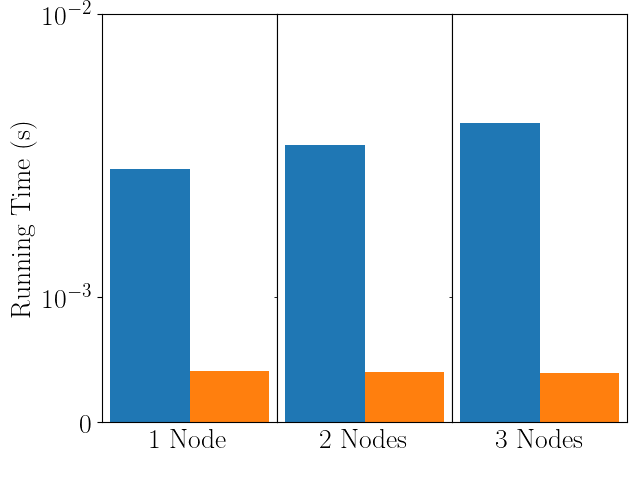
\includegraphics[scale=0.55]{images/q1-123node-none.png}}
    \caption{Running times of query 1 for 1--3 node Cassandra and Neo4J clusters, without any indexes applied.
    The blue bars represent the Cassandra queries, while the orange represent the Neo4J queries.
    Each point represents the average of 15 runs.}\label{fig:1qtyc123}
\end{figure}

In ~\autoref{fig:1qtyc123}, query 1 is plotted for Cassandra and Neo4J clusters of varying node size (1 to 3 nodes).
For brevity, only query 1 was plotted to determine if how the architecture affects query time.

The running time of Neo4J query 1 is directly proportional to the number of nodes in the cluster.
From 1 node to 2, Neo4J experiences an average increase of 1.38s in query time.
From 2 nodes to 3, Neo4J experiences an increase of 0.19s in query time.
More nodes appear to detrimental to performance here, suggesting that Neo4J may not scale out well.

On the other hand, the number of nodes in our cluster does not seem to have an effect on the running time of Cassandra
query 1.
The running times here are distributed as: $2.6\text{ms} \pm 0.5\text{ms}$.
A more significant result might be seen if a slower query were analyzed, but distributed column stores are known for
their ability to scale out.
Cassandra should provide consistent and reliable performance as more nodes are added.
